\chapter{Introduction}
\label{sec:introduction}
This chapter will introduce the subject of road and lane detection, and mixed cirticality to the reader. The problems that exist in the field and what the purpose of this degree project is.


\section{Background and problem description}
There is a global trend to make vehicles more autonomous to reduce human error and workload. Most modern vehicles include safety-critical systems where a failure can cause great damage to both humans and the environment. When the implementation is a safety-critical system it is important to be certain of the risks that are present and how to cope with them. One other increasingly important trend in the design of real-time and embedded systems is the integration of components with different criticality onto the same hardware platform \cite{burns2013mixed}.
  


The $EMC^2$ project \cite{eu} is an initiative to drive the development of "Embedded Multi-Core systems for Mixed Criticality applications in dynamic and changeable real-time environments". One focus of the project is on automotive applications for example: "Advanced Driver Assistance Systems" (ADAS). ADAS are systems designed to help the driver and to increase the safety when driving. One system is the lane detection system to help keep the car within its lanes \cite{BarHillel2014}. What differs mixed criticality systems from regular systems is that two systems with different criticality are run on the same hardware platform. One example could be to run the ADAS and the infotainment system of the vehicle on the same ECU.


"Road vehicles -functional safety", ISO 26262 is an international standard for the automotive industry regarding the electronic systems of the vehicles. ISO 26262 defines four automotive safety integrity levels, ASIL A, B, C and D. ASIL A has the lowest integrity requirements and ASIL D has the highest. The problem when implementing two applications of different criticality on the same platform is that both applications need to be certified for the level of the applications with the highest safety requirements. This means that in the case of integrating the ADAS and the infotainment system on the same hardware platform then one would need to certify the infotainment to ASIL D, which is a very tedious and thus expensive task.

If it would be possible to isolate the two applications using virtualization, it would not require any extra work on certification compared to running the applications on separate ECUs.

\section{Problem statement}
Today there is a lot of research on ADAS where everything from "Lane Departure Warning (LDW)" to "Full autonomous driving" is investigated \cite{BarHillel2014}, \cite{Yenikaya:2013:KVR:2522968.2522970}, \cite{mccall2006video}. 

However, there is a need for research about the integration of safety critical applications and non-safety critical applications on a mixed criticality platform where the two applications are isolated from each other using virtualization. For an example Autosar, which is a partnership for development of software founded by major players in the automotive industry does address mixed criticality systems in the sense that they recognize that the standards must be supported on their platforms \cite{burns2013mixed} \cite{auto}.

This thesis will investigate different techniques for road and lane detection and how they can be implemented on the RTOS of a Mixed Criticality System. 


\section{Purpose and goal}
The goal of the literature study is to give insight in the subject and answer the preliminary research question:
\begin{enumerate}  
\item What are the existing lane keeping algorithms and how do they differ from each other? In order to study the performance two parameters that could be investigated are: computation time and memory footprint.
\end{enumerate}

After the literature study is done some conclusion will be drawn and hopefully above research questions can be answered. From that an implementation phase will begin where the lane detection algorithm should be implemented on the $EMC^2$-board which consist of two operating systems on the same platform. Figure 1 shows how the software architecture of the $EMC^2$-board is set up where the Linux part is achieved through virtualization. Arm Trustzone is a hardware isolation which does not allow non-secure software from the Linux OS to access secure memory resources. This guarantees that Linux can not interfere with FMP \cite{zaki2016}. SafeG is a monitor which decides which operating system should run and when. SHAPE is a cloud for communication between different nodes. Currently SHAPE only works for the Linux OS.


\begin{figure}[H]
  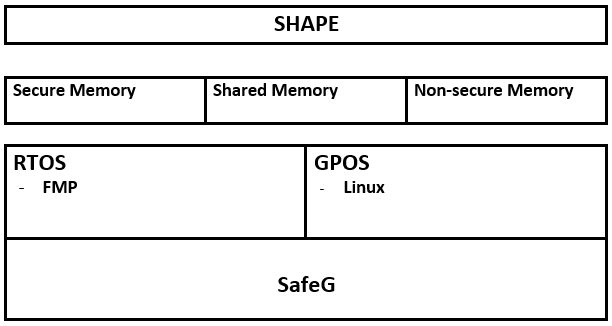
\includegraphics[scale=1]{./img/architecture.png}
  \centering
  \caption{Software architecture of the EMC2 platform}
  \label{fig:Software architecture of the EMC2 platform}
\end{figure}

The goal of the implementation phase is to evaluate how well a practical implementation of lane detection system can perform on a mixed criticality platform. Questions to be answered after the implementation:

\begin{enumerate}  
\item How can we guarantee the performance of the lane detection system?
\item How much does the speed of the convoy affect the performance of the lane detection system?
\item What are the most important parameters to evaluate when comparing different algorithms?
\end{enumerate}

\section{Goals}
In this project there are five master thesis students working together on the same demonstator. This means that there are both individual goals and team goal which do not necessarily align with each other.

\subsection{Team goal}
The team goal is to develop a demonstrator which consists of two small RC-vehicles that are supposed to group into a vehicle convoy where the first car follows a predefined path marked on the ground and the other car follows the first to demonstrate platoon driving.

\subsection{Individual goal}
The individual goal and expected outcome from this thesis is a study of existing road and lane detecting systems. Then comparing them to determine which is suitable for implementation in the safety critical system that the group is developing. The last part of the project is to implement the lane keeping algorithm on the RTOS of the mixed criticality system to demonstrate the functionality.

\section{Delimitations}
The thesis is produced at Alten.
Constrained to the Xilinx Zynq-7000 \footnote{https://www.xilinx.com/products/silicon-devices/soc/zynq-7000.html}.

The scope of this work extends to investigating lane detection and platoon driving for small vehicles operating in a constructed environment. The results will to some extent depend on the platform that the use case is built upon. In the case of objects on the track some collision avoidance system will be developed and will initially only consist of an emergency break of the vehicle.

\section{Method description}
To gain knowledge in the subject of lane and road detection systems a literature study will be performed. The literature study will give a foundation with background knowledge in the subject area and a good overview of the problems that need to be solved. From this a research problem will be formulated and goals will be developed. 

The thesis work will be of quantitative nature where experiments and testing will be done and then compared to a predefined hypothesis \cite{haakansson2013portal}. According to Håkansson \cite{haakansson2013portal} an experimental research method is often used and well suited when investigating systems performance. In this degree project the data will be measured on the developed demonstrator for confirming or rejecting a theory that was stated after the initial literature review.